% Options for packages loaded elsewhere
\PassOptionsToPackage{unicode}{hyperref}
\PassOptionsToPackage{hyphens}{url}
%
\documentclass[
]{article}
\usepackage{amsmath,amssymb}
\usepackage{iftex}
\ifPDFTeX
  \usepackage[T1]{fontenc}
  \usepackage[utf8]{inputenc}
  \usepackage{textcomp} % provide euro and other symbols
\else % if luatex or xetex
  \usepackage{unicode-math} % this also loads fontspec
  \defaultfontfeatures{Scale=MatchLowercase}
  \defaultfontfeatures[\rmfamily]{Ligatures=TeX,Scale=1}
\fi
\usepackage{lmodern}
\ifPDFTeX\else
  % xetex/luatex font selection
\fi
% Use upquote if available, for straight quotes in verbatim environments
\IfFileExists{upquote.sty}{\usepackage{upquote}}{}
\IfFileExists{microtype.sty}{% use microtype if available
  \usepackage[]{microtype}
  \UseMicrotypeSet[protrusion]{basicmath} % disable protrusion for tt fonts
}{}
\makeatletter
\@ifundefined{KOMAClassName}{% if non-KOMA class
  \IfFileExists{parskip.sty}{%
    \usepackage{parskip}
  }{% else
    \setlength{\parindent}{0pt}
    \setlength{\parskip}{6pt plus 2pt minus 1pt}}
}{% if KOMA class
  \KOMAoptions{parskip=half}}
\makeatother
\usepackage{xcolor}
\usepackage[margin= 2.00cm]{geometry}
\usepackage{color}
\usepackage{fancyvrb}
\newcommand{\VerbBar}{|}
\newcommand{\VERB}{\Verb[commandchars=\\\{\}]}
\DefineVerbatimEnvironment{Highlighting}{Verbatim}{commandchars=\\\{\}}
% Add ',fontsize=\small' for more characters per line
\usepackage{framed}
\definecolor{shadecolor}{RGB}{248,248,248}
\newenvironment{Shaded}{\begin{snugshade}}{\end{snugshade}}
\newcommand{\AlertTok}[1]{\textcolor[rgb]{0.94,0.16,0.16}{#1}}
\newcommand{\AnnotationTok}[1]{\textcolor[rgb]{0.56,0.35,0.01}{\textbf{\textit{#1}}}}
\newcommand{\AttributeTok}[1]{\textcolor[rgb]{0.13,0.29,0.53}{#1}}
\newcommand{\BaseNTok}[1]{\textcolor[rgb]{0.00,0.00,0.81}{#1}}
\newcommand{\BuiltInTok}[1]{#1}
\newcommand{\CharTok}[1]{\textcolor[rgb]{0.31,0.60,0.02}{#1}}
\newcommand{\CommentTok}[1]{\textcolor[rgb]{0.56,0.35,0.01}{\textit{#1}}}
\newcommand{\CommentVarTok}[1]{\textcolor[rgb]{0.56,0.35,0.01}{\textbf{\textit{#1}}}}
\newcommand{\ConstantTok}[1]{\textcolor[rgb]{0.56,0.35,0.01}{#1}}
\newcommand{\ControlFlowTok}[1]{\textcolor[rgb]{0.13,0.29,0.53}{\textbf{#1}}}
\newcommand{\DataTypeTok}[1]{\textcolor[rgb]{0.13,0.29,0.53}{#1}}
\newcommand{\DecValTok}[1]{\textcolor[rgb]{0.00,0.00,0.81}{#1}}
\newcommand{\DocumentationTok}[1]{\textcolor[rgb]{0.56,0.35,0.01}{\textbf{\textit{#1}}}}
\newcommand{\ErrorTok}[1]{\textcolor[rgb]{0.64,0.00,0.00}{\textbf{#1}}}
\newcommand{\ExtensionTok}[1]{#1}
\newcommand{\FloatTok}[1]{\textcolor[rgb]{0.00,0.00,0.81}{#1}}
\newcommand{\FunctionTok}[1]{\textcolor[rgb]{0.13,0.29,0.53}{\textbf{#1}}}
\newcommand{\ImportTok}[1]{#1}
\newcommand{\InformationTok}[1]{\textcolor[rgb]{0.56,0.35,0.01}{\textbf{\textit{#1}}}}
\newcommand{\KeywordTok}[1]{\textcolor[rgb]{0.13,0.29,0.53}{\textbf{#1}}}
\newcommand{\NormalTok}[1]{#1}
\newcommand{\OperatorTok}[1]{\textcolor[rgb]{0.81,0.36,0.00}{\textbf{#1}}}
\newcommand{\OtherTok}[1]{\textcolor[rgb]{0.56,0.35,0.01}{#1}}
\newcommand{\PreprocessorTok}[1]{\textcolor[rgb]{0.56,0.35,0.01}{\textit{#1}}}
\newcommand{\RegionMarkerTok}[1]{#1}
\newcommand{\SpecialCharTok}[1]{\textcolor[rgb]{0.81,0.36,0.00}{\textbf{#1}}}
\newcommand{\SpecialStringTok}[1]{\textcolor[rgb]{0.31,0.60,0.02}{#1}}
\newcommand{\StringTok}[1]{\textcolor[rgb]{0.31,0.60,0.02}{#1}}
\newcommand{\VariableTok}[1]{\textcolor[rgb]{0.00,0.00,0.00}{#1}}
\newcommand{\VerbatimStringTok}[1]{\textcolor[rgb]{0.31,0.60,0.02}{#1}}
\newcommand{\WarningTok}[1]{\textcolor[rgb]{0.56,0.35,0.01}{\textbf{\textit{#1}}}}
\usepackage{longtable,booktabs,array}
\usepackage{calc} % for calculating minipage widths
% Correct order of tables after \paragraph or \subparagraph
\usepackage{etoolbox}
\makeatletter
\patchcmd\longtable{\par}{\if@noskipsec\mbox{}\fi\par}{}{}
\makeatother
% Allow footnotes in longtable head/foot
\IfFileExists{footnotehyper.sty}{\usepackage{footnotehyper}}{\usepackage{footnote}}
\makesavenoteenv{longtable}
\usepackage{graphicx}
\makeatletter
\newsavebox\pandoc@box
\newcommand*\pandocbounded[1]{% scales image to fit in text height/width
  \sbox\pandoc@box{#1}%
  \Gscale@div\@tempa{\textheight}{\dimexpr\ht\pandoc@box+\dp\pandoc@box\relax}%
  \Gscale@div\@tempb{\linewidth}{\wd\pandoc@box}%
  \ifdim\@tempb\p@<\@tempa\p@\let\@tempa\@tempb\fi% select the smaller of both
  \ifdim\@tempa\p@<\p@\scalebox{\@tempa}{\usebox\pandoc@box}%
  \else\usebox{\pandoc@box}%
  \fi%
}
% Set default figure placement to htbp
\def\fps@figure{htbp}
\makeatother
\setlength{\emergencystretch}{3em} % prevent overfull lines
\providecommand{\tightlist}{%
  \setlength{\itemsep}{0pt}\setlength{\parskip}{0pt}}
\setcounter{secnumdepth}{5}
% definitions for citeproc citations
\NewDocumentCommand\citeproctext{}{}
\NewDocumentCommand\citeproc{mm}{%
  \begingroup\def\citeproctext{#2}\cite{#1}\endgroup}
\makeatletter
 % allow citations to break across lines
 \let\@cite@ofmt\@firstofone
 % avoid brackets around text for \cite:
 \def\@biblabel#1{}
 \def\@cite#1#2{{#1\if@tempswa , #2\fi}}
\makeatother
\newlength{\cslhangindent}
\setlength{\cslhangindent}{1.5em}
\newlength{\csllabelwidth}
\setlength{\csllabelwidth}{3em}
\newenvironment{CSLReferences}[2] % #1 hanging-indent, #2 entry-spacing
 {\begin{list}{}{%
  \setlength{\itemindent}{0pt}
  \setlength{\leftmargin}{0pt}
  \setlength{\parsep}{0pt}
  % turn on hanging indent if param 1 is 1
  \ifodd #1
   \setlength{\leftmargin}{\cslhangindent}
   \setlength{\itemindent}{-1\cslhangindent}
  \fi
  % set entry spacing
  \setlength{\itemsep}{#2\baselineskip}}}
 {\end{list}}
\usepackage{calc}
\newcommand{\CSLBlock}[1]{\hfill\break\parbox[t]{\linewidth}{\strut\ignorespaces#1\strut}}
\newcommand{\CSLLeftMargin}[1]{\parbox[t]{\csllabelwidth}{\strut#1\strut}}
\newcommand{\CSLRightInline}[1]{\parbox[t]{\linewidth - \csllabelwidth}{\strut#1\strut}}
\newcommand{\CSLIndent}[1]{\hspace{\cslhangindent}#1}
\usepackage{titling}
\pretitle{\begin{center} 
\includegraphics[width=6in,height=5in]{../images/UOW.png}\LARGE\\}
\posttitle{\end{center}}
\usepackage{setspace}
\onehalfspacing
\usepackage{fancyhdr}
\pagestyle{fancy}
\lhead{\fontsize{11pt}{11pt}\selectfont "Times New Roman"}
\fancyhead[L]{\fontsize{11}{11}\selectfont STAT950/STAT250 ASSESSMENT 03 - Sharon Van Den Berg 9251936}
\fancyhead[R]{}
\lfoot{\fontsize{11pt}{11pt}\selectfont "Serif"}
\fancyfoot[C]{\thepage}
\fancyfoot[L]{}
\usepackage{pdflscape}
\newcommand{\blandscape}{\begin{landscape}}
\newcommand{\elandscape}{\end{landscape}}
\usepackage{booktabs}
\usepackage{longtable}
\usepackage{array}
\usepackage{multirow}
\usepackage{wrapfig}
\usepackage{float}
\usepackage{colortbl}
\usepackage{pdflscape}
\usepackage{tabu}
\usepackage{threeparttable}
\usepackage{threeparttablex}
\usepackage[normalem]{ulem}
\usepackage{makecell}
\usepackage{xcolor}
\usepackage{bookmark}
\IfFileExists{xurl.sty}{\usepackage{xurl}}{} % add URL line breaks if available
\urlstyle{same}
\hypersetup{
  pdftitle={Assignment 3 - Final Report},
  pdfauthor={Sharon Van Den Berg 9251936 (stvdb914@uowmail.edu.au); School of Mathematics and Applied Statistics},
  hidelinks,
  pdfcreator={LaTeX via pandoc}}

\title{Assignment 3 - Final Report}
\usepackage{etoolbox}
\makeatletter
\providecommand{\subtitle}[1]{% add subtitle to \maketitle
  \apptocmd{\@title}{\par {\large #1 \par}}{}{}
}
\makeatother
\subtitle{Setting the environment}
\author{Sharon Van Den Berg 9251936 (\href{mailto:stvdb914@uowmail.edu.au}{\nolinkurl{stvdb914@uowmail.edu.au}}) \and School of Mathematics and Applied Statistics}
\date{26 May, 2025}

\begin{document}
\maketitle

\textbf{DECLARATION}
No part of this Assignment has been copied from anyone else, and I have not lent any part of it to anyone else. No part of this assignment has been written by generative AI.

    \vspace*{2em}\noindent
    \hfill%
    \begin{tabular}[t]{c}
        
\includegraphics[width=3cm]{../images/Sharon.png} \\
        \rule{10em}{0.5pt}\\ Sharon Van Den Berg (9251936)
    \end{tabular}%
    \hfill%
    \begin{tabular}[t]{c}
        \today \\
        \rule{10em}{0.4pt}\\ Date
    \end{tabular}

\href{https://github.com/stvdb914/DSAA811-Final-Report}{This report was made using R Markdown as a project linking to my Git account}

\newpage

\section*{Abstract}\label{abstract}
\addcontentsline{toc}{section}{Abstract}

Since the inception of the Olympic games in 1896 humans have been on a pursuit to push their minds bodies and souls to become the best of the best. They inspire the next generation to have pride not only in themselves but in their Country.

In its inception there were a small subset of sports that the competition would occur and these can be found on the left side of Table \ref{tab:SummerWinners}. Over the years the competition occurred every four years with more nations appearing and a more diverse range of sports being included. With that there are more opportunities for athletes to compete for the glory of a medal.

As a nation, it would be nice to consider a balance where a small number of athletes could be sent whilst maximizing the haul of Olympic medals.

This report aims to look at some of the past results of the games in terms of events and medals to determine if there is any clear evidence to support reducing the number of athletes, but maintaining or improving the number of medals that can be procured.

\newpage
\tableofcontents

\section*{Glossary}\label{glossary}
\addcontentsline{toc}{section}{Glossary}

\begin{longtable}[l]{>{}ll}
\toprule
Acronym & Definition\\
\midrule
\textbf{\cellcolor{gray!10}{NOC}} & \cellcolor{gray!10}{National Olympic Committee}\\
\bottomrule
\end{longtable}

\newpage

\section*{Introduction}\label{introduction}
\addcontentsline{toc}{section}{Introduction}

The Olympics has the power to drive the pride in ones nation. Bringing home a medal whether it be gold, silver or bronze brings athletes a huge sense of pride. Since the competition started in ancient Greece from 8th century BC to the 4th century AD to the common Olympic games of Summer in 1896 and Winter in 1924 to the times of today. The cost of competing and sending athletes is high. This paper looks to reduce costs but still maximizing the medals obtained.

I look into how the Olympics have changed with the number of sports that are on offer. I determine if the number of medals is proportionate to the number of athletes that compete or is it better to send less athletes but have them compete in multiple events to maximise the likelihood of obtaining medals

And finally I look into trends regarding different sports and competitors participation looking for a competitive advantage from one sport to another.

Whilst most of the analysis is done using the Summer Olympics the functions that are driving the report can and do allow analysis for Winter sports and other years over those specified within this report.

\newpage

\section*{Background}\label{background}
\addcontentsline{toc}{section}{Background}

The Olympic games was first held in Athens in 1896, with 241 athletes and 14 nations. They participated in 43 events. These events were inspired from the ancient Olympic games that were held in Greece from 8th century BC to the 4th century AD (\citeproc{ref-a2020_olympic}{History and Heritage 2020}). The list of the events for this Olympics appears in Table \ref{tab:SummerWinners}. These Olympics become known as the Summer Olympic Games.

In 1921, the decision was made to make a Winter Olympic games to cater for snow and ice sports. The data set that I obtained contains data from the 1924 Winter Olympic Games and the list of these sports can be found in Table \ref{tab:WinterWinners}.

(\citeproc{ref-OxfordStudy}{Flyvbjerg, Stewart, and Budzier 2016}) and their 2016 Olympic Study found on average it costs approx 5.2 billion US to host a Summer Olympics and 3.1 billion US to host the Winter Olympic games. This figure did not include upgrades and improvements to the hosts major infrastructure such as airports and highways.

Further costs are incurred for the opening and closing ceremonies, and medal presentations. There are three types of medals, Gold for first place, Silver for second and Bronze for third place winners. These medals are regarded as highly prestigious and brings great pride to the athlete and the host nation when they possess them.

Every athlete that competes in these games must belong to a host nation. These nations are managed by a National Olympic Committee (NOC). This body ensures that the games are run in the interest of fairness and good sportsmanship by all countries. This can be by way of sport rules and education for all involved. It is this body that is responsible for nominating their candidates interest in hosting the future games {[}a2025\_what{]}.

Due to the size of the events, they bring in many competitors and fans for the spectacle. This in turn raises the cost of travel to the host nations during the competition window. It is these costs that the non-host nation wish to minimize whilst still able to procure the most medals possible. This is the problem that this paper is looking to assist with.

(\citeproc{ref-heazlewood_2006_prediction}{Heazlewood 2006}) has some analysis regarding models to predict the optimal athlete numbers for all swimming events. This article was able to make some of these predictions, but improvements are needed to apply these results to athletics and swimming across the various distances of the races. These models are applied to results from 2004 and earlier. This article is of particular interest because of the break down of athletes into sections, mainly swimming. It could be useful to attempt to extend their results to apply it to other sports, such as athletics in summer or cross country skiing in winter. Whilst this is similar to my investigations, I feel it is at a deeper level and more specific to swimming only. I try and stay across all sports, looking for trends and medals to proportion of athletes sent to the games. I also investigate the trends with changes in the numbers of athletes sent for a particular sport.

Now that we have obtained a data set we take a look at some questions that will guide the exploration of this data.

\newpage

\section*{Research questions and aims of the project}\label{research-questions-and-aims-of-the-project}
\addcontentsline{toc}{section}{Research questions and aims of the project}

With most of the data from all the Olympic data since its inception. The main questions we need to ask is

\emph{1) Have the events of the Olympics stayed the same? What way are they different today as apposed to the inception date?}

\emph{2) Is the number of medals obtained proportionate to the number of athletes? Can we send one athlete and have them obtain twice as many medals in events as an individual athlete? Is the number of athletes on a team proportionate to the number of medals that the team can win?}

\emph{3) What are the sports that have the most events and as such the highest potential to win a medal? Has this always been the case? What are the future predictions for medal obtainment moving into the next Olympic games in both Summer and Winter Olympics?}

This report attempts to answer all the above questions in an attempt to select the optimum number of athletes, either per team or per sport to send to the Olympics to maximize the return on the number of medals obtained.

In the next section I took a look at the rational behind why this investigation is important.

\section*{Rationale}\label{rationale}
\addcontentsline{toc}{section}{Rationale}

It is no real stretch to underestimate the importance of pride that can come from winning many medals at an Olympic games. From the eyes of the country the cost to participate can be exorbitant to send one athlete, let alone an entire team of athletes. The rational for this project is to maximize the number of medals that a country can win, whilst reducing the costs of sending athletes to perform on this stage. I am looking for the optimal number of competing athletes to maximize the gold. In order to look into this problem, we can use past results in order to predict the future.

Using the data from the past we can look for trends specific to our country (or team), and across sports. We can get insights regarding the number of events that we enter to see if this is proportionate to the number of medals we can expect regarding to the team or sport. Furthermore we can get insights regarding sports with waning interests or declining numbers and vice-versa.

Getting a dossier of this information, a nation will be well equipped to send the appropriate team numbers to the next games, confidently reducing travel and stay costs for the athlete, whilst still able to procure the most medals possible. This is a win for the athletes and the country pride that is associated with a win on a global stage.

In the next section we take a look into the data descriptions, and how the data was obtained.

\newpage

\section*{Data Description}\label{data-description}
\addcontentsline{toc}{section}{Data Description}

The (\citeproc{ref-bansal_2021_olympics_}{Bansal 2021}) data set called ``Olympics\_'' was compiled by ``Harsh Bansal'' and was last updated 4 years ago. The dataset was uploaded and sourced from Kaggle (\citeproc{ref-keating_2025_kaggle}{Keating et al. 2025}). According to the site, there is only one owner with no DOI Citation, provenance or license. The restriction on the data is placed on it by Kaggle by way of citation of the owner ``Harsh Bansal''. I am using this data at my own risk as it has not been authenticated or carefully curated.

The dataset contains 4 files, ``athlete\_events\_data\_dictionary.csv'' contains 15 observations of 2 variables, ``country\_definitions.csv'' contains 230 observations of 3 variables, ``country\_definitions\_data\_dictionary.csv'' contains 3 observations of 2 variables, and ``athlete\_events.csv'' containing 271,116 observations of 15 variables.

The ``athlete\_events.csv'' file contains all athlete information of all the Olympic games dating from 1896 summer games and 1924 winter games up to and including the 2016 summer Olympic games. The following table outlines the variables contained within the set.

\begin{longtable}[t]{ll}
\toprule
Field & Description\\
\midrule
ID & Unique number for each athlete\\
Name & Athlete's name\\
Sex & Male (M) or Female (F)\\
Age & Integer\\
Height & In centimeters\\
\addlinespace
Weight & In kilograms\\
Team & Team name\\
NOC & National Olympic Committee 3-letter code\\
Games & Year and season\\
Year & Integer\\
\addlinespace
Season & Summer or Winter\\
City & Host city\\
Sport & Sport\\
Event & Event\\
Medal & Gold, Silver, Bronze, or NA\\
\bottomrule
\end{longtable}

The research will center around the ID, NOC, Season, Year, Sport and Medals. I am trying to work out if sending more athletes equates to more medals. If I can isolate what year there is differences in the medal tally for some countries we can pinpoint what if anything was occurring in that country at the time. This may give insight to the specific number of athletes required to send to the games to capitalize on medals.

In the athletes table there is a field called NOC which is the National Olympic City code that links to the country definitions that will allow for better groupings of data by country when linked to each other.

To represent the data on a world map I needed to obtain another data set of data that contained the longitude and latitude. This data set was obtained from (\citeproc{ref-a262588213843476_2021_countries}{Ferlet 2021}) and contained one file, ``country-coord.csv''. It was sourced from Github and returned to Tadas Tamošauskas who provided the data set for cleaning. The set is experimental, but provides enough information to roughly plot the Olympic data on a map. It contains six variables. The three that are needed to plot the data points are Alpha-3 code that allows you to link to the NOC codes, latitude (average), and longitude (average). With this data we can obtain an image of what countries have competed in an Olympic games as seen in Figure \ref{fig:OlympicAll}

\begin{figure}
\centering
\pandocbounded{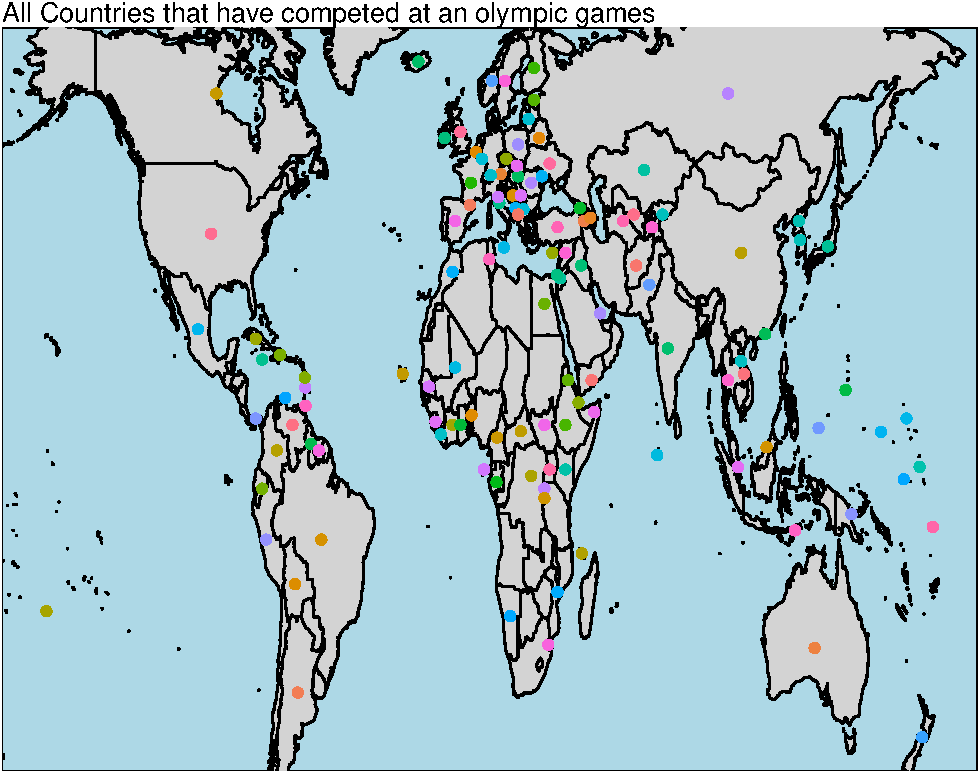
\includegraphics[keepaspectratio]{C:/Final/report/DSAA811_Final_files/figure-latex/OlympicAll-1.pdf}}
\caption{\label{fig:OlympicAll}Mapping the NOC codes to longitude and latitude points on the world map}
\end{figure}

Whilst working with this data set, and considering the questions that are being asked. The categories that are most relevant in this data set are all categorical variables, that are quantified with counts to extrapolate unique athlete ID's, or Team members, to counts of medals in all categories, gold, silver, bronze or no medal awarded. For this reason I have factored all the categorical data for ease of use.

In the next section I take a look at some of the tables and figures that can answer the questions that arose in Research Questions which will guide any conclusions that I come up with to answer them.

\newpage

\section*{Exploritory data analysis}\label{exploritory-data-analysis}
\addcontentsline{toc}{section}{Exploritory data analysis}

When loading in the data I have determined from the events table, the variables ID, Team, NOC, Season, Sport, and Medals are all factor variables and needed to be coded this way in R. These are the variables that the investigation is centered around.

Every line in the data set represents an event. It contains all the athlete competitors if they win or not. Therefor to get quantifiable data I need to use counts to gather a lot of my numerical data.

Looking into \emph{1) Have the events of the Olympics stayed the same? What way are they different today as apposed to the inception date?} I begin with a specific year of an Olympic games. Table \ref{tab:SummerWinners} takes a look at the number of medals available for the inception data of the summer Olympics in 1896 as apposed to the last summer games in the data set of 2016. On the left side we can see that there are only 9 sports, and 143 medals. This is correct to the reported data mentioned in (\citeproc{ref-a2020_olympic}{History and Heritage 2020}). On the right side we can see that in 2016 there are now a lot more sports on offer, over 30 types. Interestingly all the sports that existed in the summer games in 1896 are still being represented in the Summer Olympic Games in 2016.

A similar story can be said about the winter Olympics when looking at Table \ref{tab:WinterWinners}. In 1924, on the left side there are ten sports. On the right there are fifteen sports being competed in in 2014. There are some sports that are no longer competed in from the 1924 such as Military Ski Patrol.

Whilst there are a lot more medals on offer in the later Olympics, the dynamic of the Olympics has changed dramatically through the years. This poses a problem with the investigation because there are now new sports that were not even conceived in the early games. Even though there are new sporting events there is no evidence as to how many athletes we should send to capitalise on the medals.

\begin{table}
\centering\caption{\label{tab:SummerWinners}Number of medal winners in 1896 versus 2016 Summer Olympic Games}

\centering
\begin{tabular}[t]{lr}
\toprule
Sport & \vphantom{1} Medals\_Given\\
\midrule
\cellcolor{gray!10}{Athletics} & \cellcolor{gray!10}{37}\\
Cycling & 16\\
\cellcolor{gray!10}{Fencing} & \cellcolor{gray!10}{9}\\
Gymnastics & 37\\
\cellcolor{gray!10}{Shooting} & \cellcolor{gray!10}{15}\\
\addlinespace
Swimming & 10\\
\cellcolor{gray!10}{Tennis} & \cellcolor{gray!10}{10}\\
Weightlifting & 6\\
\cellcolor{gray!10}{Wrestling} & \cellcolor{gray!10}{3}\\
\bottomrule
\end{tabular}
\centering
\begin{tabular}[t]{lr}
\toprule
Sport & Medals\_Given\\
\midrule
\cellcolor{gray!10}{Archery} & \cellcolor{gray!10}{24}\\
Athletics & 192\\
\cellcolor{gray!10}{Badminton} & \cellcolor{gray!10}{24}\\
Basketball & 72\\
\cellcolor{gray!10}{Beach Volleyball} & \cellcolor{gray!10}{12}\\
\addlinespace
Boxing & 51\\
\cellcolor{gray!10}{Canoeing} & \cellcolor{gray!10}{82}\\
Cycling & 84\\
\cellcolor{gray!10}{Diving} & \cellcolor{gray!10}{36}\\
Equestrianism & 45\\
\addlinespace
\cellcolor{gray!10}{Fencing} & \cellcolor{gray!10}{65}\\
Football & 106\\
\cellcolor{gray!10}{Golf} & \cellcolor{gray!10}{6}\\
Gymnastics & 66\\
\cellcolor{gray!10}{Handball} & \cellcolor{gray!10}{89}\\
\addlinespace
Hockey & 99\\
\cellcolor{gray!10}{Judo} & \cellcolor{gray!10}{56}\\
Modern Pentathlon & 6\\
\cellcolor{gray!10}{Rhythmic Gymnastics} & \cellcolor{gray!10}{18}\\
Rowing & 144\\
\addlinespace
\cellcolor{gray!10}{Rugby Sevens} & \cellcolor{gray!10}{74}\\
Sailing & 45\\
\cellcolor{gray!10}{Shooting} & \cellcolor{gray!10}{45}\\
Swimming & 191\\
\cellcolor{gray!10}{Synchronized Swimming} & \cellcolor{gray!10}{32}\\
\addlinespace
Table Tennis & 24\\
\cellcolor{gray!10}{Taekwondo} & \cellcolor{gray!10}{32}\\
Tennis & 24\\
\cellcolor{gray!10}{Trampolining} & \cellcolor{gray!10}{6}\\
Triathlon & 6\\
\addlinespace
\cellcolor{gray!10}{Volleyball} & \cellcolor{gray!10}{72}\\
Water Polo & 78\\
\cellcolor{gray!10}{Weightlifting} & \cellcolor{gray!10}{45}\\
Wrestling & 72\\
\bottomrule
\end{tabular}
\end{table}
\newpage

\begin{table}
\centering\caption{\label{tab:WinterWinners}Number of medal winners in 1924 versus 2014 Winter Olympic Games}

\centering
\begin{tabular}[t]{lr}
\toprule
Sport & \vphantom{1} Medals\_Given\\
\midrule
\cellcolor{gray!10}{Alpinism} & \cellcolor{gray!10}{21}\\
Bobsleigh & 13\\
\cellcolor{gray!10}{Cross Country Skiing} & \cellcolor{gray!10}{6}\\
Curling & 16\\
\cellcolor{gray!10}{Figure Skating} & \cellcolor{gray!10}{12}\\
\addlinespace
Ice Hockey & 28\\
\cellcolor{gray!10}{Military Ski Patrol} & \cellcolor{gray!10}{12}\\
Nordic Combined & 3\\
\cellcolor{gray!10}{Ski Jumping} & \cellcolor{gray!10}{3}\\
Speed Skating & 16\\
\bottomrule
\end{tabular}
\centering
\begin{tabular}[t]{lr}
\toprule
\cellcolor{gray!10}{Sport} & \cellcolor{gray!10}{Medals\_Given}\\
\midrule
Alpine Skiing & 31\\
\cellcolor{gray!10}{Biathlon} & \cellcolor{gray!10}{60}\\
Bobsleigh & 24\\
\cellcolor{gray!10}{Cross Country Skiing} & \cellcolor{gray!10}{60}\\
Curling & 24\\
\addlinespace
\cellcolor{gray!10}{Figure Skating} & \cellcolor{gray!10}{45}\\
Freestyle Skiing & 30\\
\cellcolor{gray!10}{Ice Hockey} & \cellcolor{gray!10}{130}\\
Luge & 24\\
\cellcolor{gray!10}{Nordic Combined} & \cellcolor{gray!10}{18}\\
\addlinespace
Short Track Speed Skating & 43\\
\cellcolor{gray!10}{Skeleton} & \cellcolor{gray!10}{6}\\
Ski Jumping & 21\\
\cellcolor{gray!10}{Snowboarding} & \cellcolor{gray!10}{30}\\
Speed Skating & 51\\
\bottomrule
\end{tabular}
\end{table}

\newpage

Further to knowing how many events are competed in each sport, we can get a breakdown of the medal tally as seen in Table \ref{tab:SummerBreakDownWinners1}. In this table we can see the number of Gold, Silver and Bronze medals that are awarded to each team for the Summer Olympics in 1986. We can also see how many events each team participated. Similarly we can perform the same query and compare the tables for the Olympics in 2016 for the top 30 teams in \ref{tab:SummerBreakDownWinners2}. The main difference in these two tables is that as the years progressed there are now more teams engaging in the endevour to win medals.

\begin{table}[H]
\centering
\caption{\label{tab:SummerBreakDownWinners1}Medal allocation for 1896 Summer Olympic Games}
\centering
\fontsize{7}{9}\selectfont
\begin{tabular}[t]{lrrrrr}
\toprule
Team & Gold & Silver & Bronze & Events & Medals\\
\midrule
\cellcolor{gray!10}{Greece} & \cellcolor{gray!10}{10} & \cellcolor{gray!10}{16} & \cellcolor{gray!10}{18} & \cellcolor{gray!10}{140} & \cellcolor{gray!10}{44}\\
Germany & 24 & 5 & 2 & 93 & 31\\
\cellcolor{gray!10}{United States} & \cellcolor{gray!10}{11} & \cellcolor{gray!10}{7} & \cellcolor{gray!10}{2} & \cellcolor{gray!10}{27} & \cellcolor{gray!10}{20}\\
France & 5 & 4 & 2 & 26 & 11\\
\cellcolor{gray!10}{Great Britain} & \cellcolor{gray!10}{2} & \cellcolor{gray!10}{3} & \cellcolor{gray!10}{2} & \cellcolor{gray!10}{23} & \cellcolor{gray!10}{7}\\
\addlinespace
Denmark & 1 & 2 & 3 & 15 & 6\\
\cellcolor{gray!10}{Hungary} & \cellcolor{gray!10}{2} & \cellcolor{gray!10}{1} & \cellcolor{gray!10}{3} & \cellcolor{gray!10}{18} & \cellcolor{gray!10}{6}\\
Austria & 2 & 1 & 2 & 8 & 5\\
\cellcolor{gray!10}{Switzerland} & \cellcolor{gray!10}{1} & \cellcolor{gray!10}{2} & \cellcolor{gray!10}{0} & \cellcolor{gray!10}{8} & \cellcolor{gray!10}{3}\\
Australia & 2 & 0 & 0 & 4 & 2\\
\addlinespace
\cellcolor{gray!10}{Australia/Great Britain} & \cellcolor{gray!10}{0} & \cellcolor{gray!10}{0} & \cellcolor{gray!10}{2} & \cellcolor{gray!10}{2} & \cellcolor{gray!10}{2}\\
Ethnikos Gymnastikos Syllogos & 0 & 0 & 2 & 2 & 2\\
\cellcolor{gray!10}{Great Britain/Germany} & \cellcolor{gray!10}{2} & \cellcolor{gray!10}{0} & \cellcolor{gray!10}{0} & \cellcolor{gray!10}{2} & \cellcolor{gray!10}{2}\\
Greece-1 & 0 & 2 & 0 & 2 & 2\\
\cellcolor{gray!10}{Greece-2} & \cellcolor{gray!10}{0} & \cellcolor{gray!10}{0} & \cellcolor{gray!10}{0} & \cellcolor{gray!10}{2} & \cellcolor{gray!10}{0}\\
\addlinespace
Greece-3 & 0 & 0 & 0 & 2 & 0\\
\cellcolor{gray!10}{Italy} & \cellcolor{gray!10}{0} & \cellcolor{gray!10}{0} & \cellcolor{gray!10}{0} & \cellcolor{gray!10}{1} & \cellcolor{gray!10}{0}\\
Sweden & 0 & 0 & 0 & 5 & 0\\
\bottomrule
\end{tabular}
\end{table}

\newpage

\begin{table}[H]
\centering
\caption{\label{tab:SummerBreakDownWinners2}Medal allocation for 2016 Summer Olympic Games for the top 30 teams}
\centering
\fontsize{7}{9}\selectfont
\begin{tabular}[t]{lrrrrr}
\toprule
Team & Gold & Silver & Bronze & Events & Medals\\
\midrule
\cellcolor{gray!10}{United States} & \cellcolor{gray!10}{137} & \cellcolor{gray!10}{52} & \cellcolor{gray!10}{67} & \cellcolor{gray!10}{699} & \cellcolor{gray!10}{256}\\
Germany & 47 & 43 & 67 & 528 & 157\\
\cellcolor{gray!10}{Great Britain} & \cellcolor{gray!10}{64} & \cellcolor{gray!10}{55} & \cellcolor{gray!10}{26} & \cellcolor{gray!10}{470} & \cellcolor{gray!10}{145}\\
Russia & 50 & 28 & 35 & 398 & 113\\
\cellcolor{gray!10}{China} & \cellcolor{gray!10}{44} & \cellcolor{gray!10}{30} & \cellcolor{gray!10}{35} & \cellcolor{gray!10}{483} & \cellcolor{gray!10}{109}\\
\addlinespace
France & 20 & 55 & 21 & 504 & 96\\
\cellcolor{gray!10}{Australia} & \cellcolor{gray!10}{23} & \cellcolor{gray!10}{34} & \cellcolor{gray!10}{25} & \cellcolor{gray!10}{510} & \cellcolor{gray!10}{82}\\
Italy & 8 & 38 & 24 & 395 & 70\\
\cellcolor{gray!10}{Canada} & \cellcolor{gray!10}{4} & \cellcolor{gray!10}{4} & \cellcolor{gray!10}{61} & \cellcolor{gray!10}{397} & \cellcolor{gray!10}{69}\\
Japan & 17 & 13 & 34 & 436 & 64\\
\addlinespace
\cellcolor{gray!10}{Serbia} & \cellcolor{gray!10}{14} & \cellcolor{gray!10}{27} & \cellcolor{gray!10}{13} & \cellcolor{gray!10}{127} & \cellcolor{gray!10}{54}\\
Brazil & 34 & 6 & 6 & 571 & 46\\
\cellcolor{gray!10}{Netherlands} & \cellcolor{gray!10}{9} & \cellcolor{gray!10}{25} & \cellcolor{gray!10}{11} & \cellcolor{gray!10}{321} & \cellcolor{gray!10}{45}\\
Spain & 7 & 19 & 17 & 353 & 43\\
\cellcolor{gray!10}{Denmark} & \cellcolor{gray!10}{15} & \cellcolor{gray!10}{10} & \cellcolor{gray!10}{16} & \cellcolor{gray!10}{143} & \cellcolor{gray!10}{41}\\
\addlinespace
New Zealand & 6 & 25 & 5 & 232 & 36\\
\cellcolor{gray!10}{Jamaica} & \cellcolor{gray!10}{11} & \cellcolor{gray!10}{17} & \cellcolor{gray!10}{2} & \cellcolor{gray!10}{77} & \cellcolor{gray!10}{30}\\
Sweden & 2 & 23 & 3 & 186 & 28\\
\cellcolor{gray!10}{Croatia} & \cellcolor{gray!10}{7} & \cellcolor{gray!10}{15} & \cellcolor{gray!10}{2} & \cellcolor{gray!10}{93} & \cellcolor{gray!10}{24}\\
South Korea & 13 & 3 & 8 & 255 & 24\\
\addlinespace
\cellcolor{gray!10}{South Africa} & \cellcolor{gray!10}{2} & \cellcolor{gray!10}{7} & \cellcolor{gray!10}{14} & \cellcolor{gray!10}{155} & \cellcolor{gray!10}{23}\\
Argentina & 21 & 1 & 0 & 228 & 22\\
\cellcolor{gray!10}{Hungary} & \cellcolor{gray!10}{12} & \cellcolor{gray!10}{3} & \cellcolor{gray!10}{7} & \cellcolor{gray!10}{204} & \cellcolor{gray!10}{22}\\
Belgium & 2 & 17 & 2 & 138 & 21\\
\cellcolor{gray!10}{Norway} & \cellcolor{gray!10}{0} & \cellcolor{gray!10}{0} & \cellcolor{gray!10}{19} & \cellcolor{gray!10}{77} & \cellcolor{gray!10}{19}\\
\addlinespace
Azerbaijan & 1 & 7 & 10 & 69 & 18\\
\cellcolor{gray!10}{Kazakhstan} & \cellcolor{gray!10}{3} & \cellcolor{gray!10}{5} & \cellcolor{gray!10}{10} & \cellcolor{gray!10}{123} & \cellcolor{gray!10}{18}\\
Nigeria & 0 & 0 & 18 & 77 & 18\\
\cellcolor{gray!10}{Poland} & \cellcolor{gray!10}{3} & \cellcolor{gray!10}{3} & \cellcolor{gray!10}{10} & \cellcolor{gray!10}{285} & \cellcolor{gray!10}{16}\\
Romania & 4 & 2 & 10 & 117 & 16\\
\bottomrule
\end{tabular}
\end{table}

Similarly, we can view the breakdown of medals per team for the Winter Olympics in 1924 in \ref{tab:WinterBreakDownWinners1} and for the top 30 teams in the 2014 winter Olympics \ref{tab:WinterBreakDownWinners2}.

On closer observations we can see that in 1896 Summer Olympics Egypt participated in 140 events and this translated to 44 medals. Of that 10 were gold, 16 were silver and 18 were bronze. Whereas in the same year Sweeden entered 5 events but did not win any medals. Seeing that there are an increasing variety of sports and events makes making a decision regarding the optimal athletes difficult to discern. Seeing the proportions of events entered as apposed to the take home medals leads me to the leads to the next question, \emph{2) Is the number of medals obtained proportionate to the number of athletes? Can we send one athlete and have them obtain twice as many medals in events as an individual athlete? Is the number of athletes on a team proportionate to the number of medals that the team can win?}

\newpage

\begin{table}[H]
\centering
\caption{\label{tab:WinterBreakDownWinners1}Medal allocation for 1924 Winter Olympic Games}
\centering
\fontsize{7}{9}\selectfont
\begin{tabular}[t]{lrrrrrr}
\toprule
Team & None & Gold & Silver & Bronze & TotalEvents & TotalMedals\\
\midrule
\cellcolor{gray!10}{Great Britain} & \cellcolor{gray!10}{11} & \cellcolor{gray!10}{16} & \cellcolor{gray!10}{0} & \cellcolor{gray!10}{11} & \cellcolor{gray!10}{38} & \cellcolor{gray!10}{27}\\
Norway & 19 & 4 & 7 & 6 & 36 & 17\\
\cellcolor{gray!10}{Finland} & \cellcolor{gray!10}{18} & \cellcolor{gray!10}{4} & \cellcolor{gray!10}{8} & \cellcolor{gray!10}{3} & \cellcolor{gray!10}{33} & \cellcolor{gray!10}{15}\\
United States & 29 & 1 & 10 & 1 & 41 & 12\\
\cellcolor{gray!10}{Canada} & \cellcolor{gray!10}{8} & \cellcolor{gray!10}{9} & \cellcolor{gray!10}{0} & \cellcolor{gray!10}{0} & \cellcolor{gray!10}{17} & \cellcolor{gray!10}{9}\\
\addlinespace
Sweden & 32 & 1 & 8 & 0 & 41 & 9\\
\cellcolor{gray!10}{France} & \cellcolor{gray!10}{48} & \cellcolor{gray!10}{0} & \cellcolor{gray!10}{0} & \cellcolor{gray!10}{8} & \cellcolor{gray!10}{56} & \cellcolor{gray!10}{8}\\
India & 0 & 7 & 0 & 0 & 7 & 7\\
\cellcolor{gray!10}{Belgium-1} & \cellcolor{gray!10}{0} & \cellcolor{gray!10}{0} & \cellcolor{gray!10}{0} & \cellcolor{gray!10}{5} & \cellcolor{gray!10}{5} & \cellcolor{gray!10}{5}\\
Switzerland & 26 & 4 & 0 & 1 & 31 & 5\\
\addlinespace
\cellcolor{gray!10}{Austria} & \cellcolor{gray!10}{0} & \cellcolor{gray!10}{3} & \cellcolor{gray!10}{1} & \cellcolor{gray!10}{0} & \cellcolor{gray!10}{4} & \cellcolor{gray!10}{4}\\
Great Britain-1 & 2 & 0 & 4 & 0 & 6 & 4\\
\cellcolor{gray!10}{Switzerland-1} & \cellcolor{gray!10}{0} & \cellcolor{gray!10}{4} & \cellcolor{gray!10}{0} & \cellcolor{gray!10}{0} & \cellcolor{gray!10}{4} & \cellcolor{gray!10}{4}\\
France-1 & 4 & 0 & 0 & 2 & 6 & 2\\
\cellcolor{gray!10}{Australia} & \cellcolor{gray!10}{0} & \cellcolor{gray!10}{1} & \cellcolor{gray!10}{0} & \cellcolor{gray!10}{0} & \cellcolor{gray!10}{1} & \cellcolor{gray!10}{1}\\
\addlinespace
Nepal & 0 & 1 & 0 & 0 & 1 & 1\\
\cellcolor{gray!10}{Belgium} & \cellcolor{gray!10}{27} & \cellcolor{gray!10}{0} & \cellcolor{gray!10}{0} & \cellcolor{gray!10}{0} & \cellcolor{gray!10}{27} & \cellcolor{gray!10}{0}\\
Czechoslovakia & 31 & 0 & 0 & 0 & 31 & 0\\
\cellcolor{gray!10}{France-2} & \cellcolor{gray!10}{6} & \cellcolor{gray!10}{0} & \cellcolor{gray!10}{0} & \cellcolor{gray!10}{0} & \cellcolor{gray!10}{6} & \cellcolor{gray!10}{0}\\
Great Britain-2 & 6 & 0 & 0 & 0 & 6 & 0\\
\addlinespace
\cellcolor{gray!10}{Hungary} & \cellcolor{gray!10}{6} & \cellcolor{gray!10}{0} & \cellcolor{gray!10}{0} & \cellcolor{gray!10}{0} & \cellcolor{gray!10}{6} & \cellcolor{gray!10}{0}\\
Italy & 14 & 0 & 0 & 0 & 14 & 0\\
\cellcolor{gray!10}{Italy-1} & \cellcolor{gray!10}{5} & \cellcolor{gray!10}{0} & \cellcolor{gray!10}{0} & \cellcolor{gray!10}{0} & \cellcolor{gray!10}{5} & \cellcolor{gray!10}{0}\\
Italy-2 & 5 & 0 & 0 & 0 & 5 & 0\\
\cellcolor{gray!10}{Latvia} & \cellcolor{gray!10}{7} & \cellcolor{gray!10}{0} & \cellcolor{gray!10}{0} & \cellcolor{gray!10}{0} & \cellcolor{gray!10}{7} & \cellcolor{gray!10}{0}\\
\addlinespace
Poland & 15 & 0 & 0 & 0 & 15 & 0\\
\cellcolor{gray!10}{Switzerland-2} & \cellcolor{gray!10}{4} & \cellcolor{gray!10}{0} & \cellcolor{gray!10}{0} & \cellcolor{gray!10}{0} & \cellcolor{gray!10}{4} & \cellcolor{gray!10}{0}\\
Yugoslavia & 7 & 0 & 0 & 0 & 7 & 0\\
\bottomrule
\end{tabular}
\end{table}

\begin{table}[H]
\centering
\caption{\label{tab:WinterBreakDownWinners2}Medal allocation for 2014 Winter Olympic Games for the top 30 teams}
\centering
\fontsize{7}{9}\selectfont
\begin{tabular}[t]{lrrrrrr}
\toprule
Team & None & Gold & Silver & Bronze & TotalEvents & TotalMedals\\
\midrule
\cellcolor{gray!10}{Canada} & \cellcolor{gray!10}{241} & \cellcolor{gray!10}{57} & \cellcolor{gray!10}{20} & \cellcolor{gray!10}{5} & \cellcolor{gray!10}{323} & \cellcolor{gray!10}{82}\\
Russia & 261 & 25 & 20 & 11 & 317 & 56\\
\cellcolor{gray!10}{United States} & \cellcolor{gray!10}{281} & \cellcolor{gray!10}{8} & \cellcolor{gray!10}{28} & \cellcolor{gray!10}{16} & \cellcolor{gray!10}{333} & \cellcolor{gray!10}{52}\\
Sweden & 97 & 8 & 32 & 11 & 148 & 51\\
\cellcolor{gray!10}{Norway} & \cellcolor{gray!10}{183} & \cellcolor{gray!10}{18} & \cellcolor{gray!10}{5} & \cellcolor{gray!10}{13} & \cellcolor{gray!10}{219} & \cellcolor{gray!10}{36}\\
\addlinespace
Finland & 114 & 2 & 7 & 24 & 147 & 33\\
\cellcolor{gray!10}{Germany} & \cellcolor{gray!10}{203} & \cellcolor{gray!10}{13} & \cellcolor{gray!10}{12} & \cellcolor{gray!10}{7} & \cellcolor{gray!10}{235} & \cellcolor{gray!10}{32}\\
Netherlands & 53 & 13 & 7 & 9 & 82 & 29\\
\cellcolor{gray!10}{Switzerland} & \cellcolor{gray!10}{187} & \cellcolor{gray!10}{6} & \cellcolor{gray!10}{2} & \cellcolor{gray!10}{20} & \cellcolor{gray!10}{215} & \cellcolor{gray!10}{28}\\
Austria & 184 & 4 & 10 & 11 & 209 & 25\\
\addlinespace
\cellcolor{gray!10}{France} & \cellcolor{gray!10}{171} & \cellcolor{gray!10}{4} & \cellcolor{gray!10}{4} & \cellcolor{gray!10}{10} & \cellcolor{gray!10}{189} & \cellcolor{gray!10}{18}\\
Italy & 201 & 0 & 2 & 12 & 215 & 14\\
\cellcolor{gray!10}{South Korea} & \cellcolor{gray!10}{104} & \cellcolor{gray!10}{7} & \cellcolor{gray!10}{5} & \cellcolor{gray!10}{2} & \cellcolor{gray!10}{118} & \cellcolor{gray!10}{14}\\
China & 93 & 3 & 4 & 5 & 105 & 12\\
\cellcolor{gray!10}{Czech Republic} & \cellcolor{gray!10}{168} & \cellcolor{gray!10}{2} & \cellcolor{gray!10}{7} & \cellcolor{gray!10}{2} & \cellcolor{gray!10}{179} & \cellcolor{gray!10}{11}\\
\addlinespace
Japan & 160 & 1 & 4 & 6 & 171 & 11\\
\cellcolor{gray!10}{Poland} & \cellcolor{gray!10}{138} & \cellcolor{gray!10}{4} & \cellcolor{gray!10}{4} & \cellcolor{gray!10}{3} & \cellcolor{gray!10}{149} & \cellcolor{gray!10}{11}\\
Great Britain & 60 & 1 & 4 & 5 & 70 & 10\\
\cellcolor{gray!10}{Russia-1} & \cellcolor{gray!10}{4} & \cellcolor{gray!10}{8} & \cellcolor{gray!10}{0} & \cellcolor{gray!10}{2} & \cellcolor{gray!10}{14} & \cellcolor{gray!10}{10}\\
United States-1 & 4 & 2 & 2 & 6 & 14 & 10\\
\addlinespace
\cellcolor{gray!10}{Slovenia} & \cellcolor{gray!10}{108} & \cellcolor{gray!10}{2} & \cellcolor{gray!10}{2} & \cellcolor{gray!10}{4} & \cellcolor{gray!10}{116} & \cellcolor{gray!10}{8}\\
Belarus & 66 & 5 & 0 & 1 & 72 & 6\\
\cellcolor{gray!10}{Latvia-1} & \cellcolor{gray!10}{2} & \cellcolor{gray!10}{0} & \cellcolor{gray!10}{4} & \cellcolor{gray!10}{2} & \cellcolor{gray!10}{8} & \cellcolor{gray!10}{6}\\
Latvia & 61 & 0 & 1 & 4 & 66 & 5\\
\cellcolor{gray!10}{Ukraine} & \cellcolor{gray!10}{96} & \cellcolor{gray!10}{4} & \cellcolor{gray!10}{0} & \cellcolor{gray!10}{1} & \cellcolor{gray!10}{101} & \cellcolor{gray!10}{5}\\
\addlinespace
Canada-1 & 8 & 2 & 2 & 0 & 12 & 4\\
\cellcolor{gray!10}{Germany-1} & \cellcolor{gray!10}{10} & \cellcolor{gray!10}{2} & \cellcolor{gray!10}{0} & \cellcolor{gray!10}{2} & \cellcolor{gray!10}{14} & \cellcolor{gray!10}{4}\\
Australia & 81 & 0 & 2 & 1 & 84 & 3\\
\cellcolor{gray!10}{Austria-1} & \cellcolor{gray!10}{0} & \cellcolor{gray!10}{0} & \cellcolor{gray!10}{2} & \cellcolor{gray!10}{0} & \cellcolor{gray!10}{2} & \cellcolor{gray!10}{2}\\
Russia-2 & 12 & 0 & 2 & 0 & 14 & 2\\
\bottomrule
\end{tabular}
\end{table}

\newpage

Taking a look at the Figure \ref{fig:medalProp} alongside the Table \ref{tab:SummerBreakDownWinners1} we can see the proportion of medals won in comparison to the number of events the team entered in. We can see that Greece has had a 7\% turn around of all events entered that brought in the gold medal, whereas 69\% of the time they come up empty handed. Australia brought home the gold in 50\% of the events that they entered. Sweeden, Italy, Greece-3 and Greece 2 did not win any of the events that they entered. Great Britain/Germany won the gold medal in every event entered. Figure \ref{fig:medalProp1} staggers the bar chart and neither of these graphs are easy to read. Both, however highlight a quick reference showing that the more events participated in does not lead to more medals.

\begin{figure}
\centering
\pandocbounded{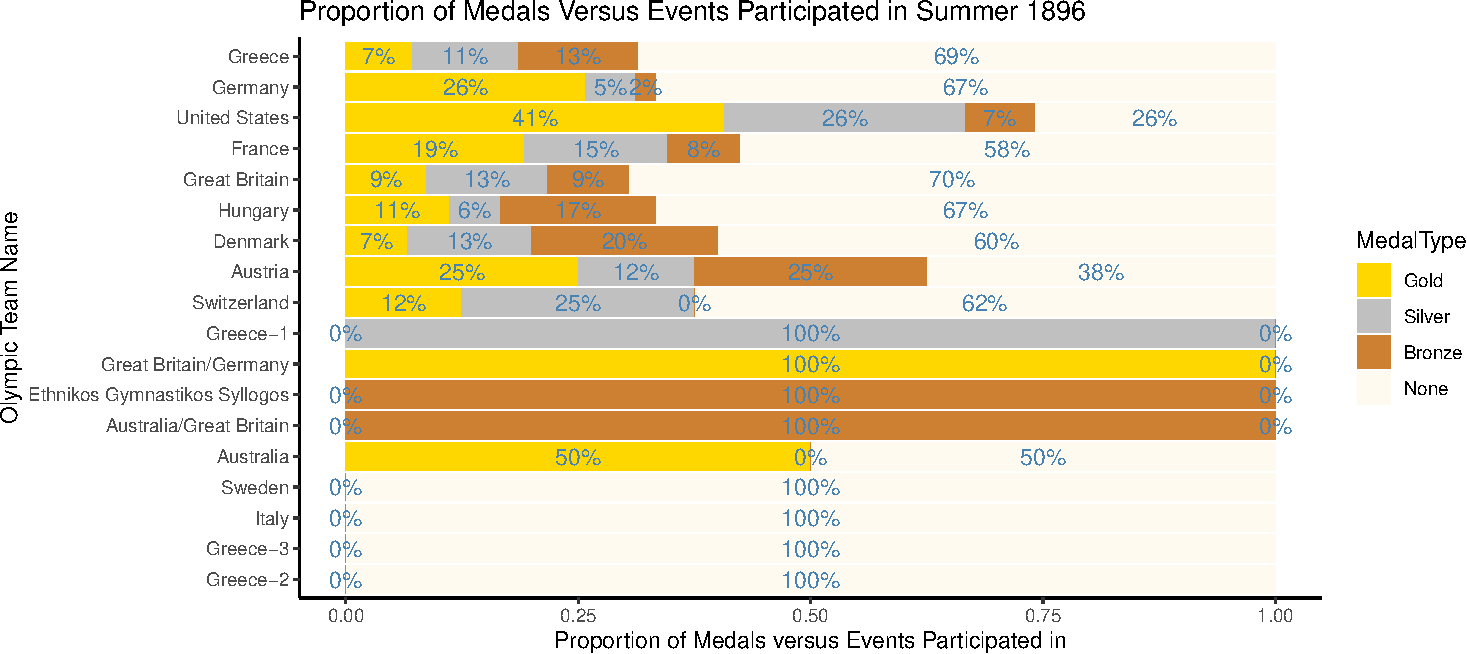
\includegraphics[keepaspectratio]{C:/Final/report/DSAA811_Final_files/figure-latex/medalProp-1.pdf}}
\caption{\label{fig:medalProp}Proportion of medals in relation to the events entered by teams in the Summer 1896 Olympics}
\end{figure}

\begin{figure}
\centering
\pandocbounded{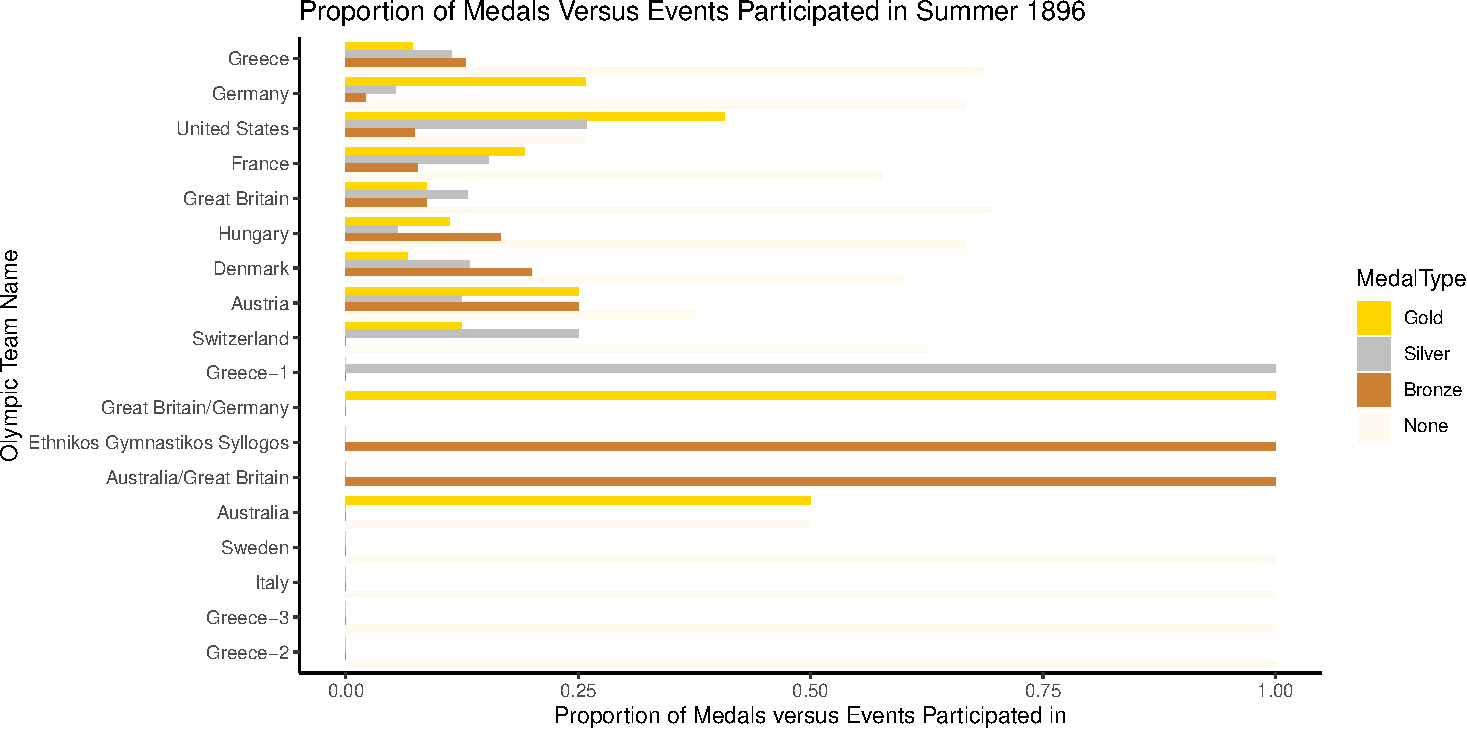
\includegraphics[keepaspectratio]{C:/Final/report/DSAA811_Final_files/figure-latex/medalProp1-1.pdf}}
\caption{\label{fig:medalProp1}Proportion of medals in relation to the events entered by teams in the Summer 1896 Olympics}
\end{figure}

Similarly we can examine the results for the Winter olympics. In Figure \ref{fig:medalProp3} and following Table \ref{tab:WinterBreakDownWinners1} we can see that Great Brittain won the most medals with 27 out of the 38 events. This means that 29\% of the events did not medal. 42\% of their events medalled with a gold. Australia and Nepal won all their events gaining gold. Figure \ref{fig:medalProp4} stacks these proportions side by side.

The problem I am facing with these proportions is that there is no information regarding the actual team sizes. In the dataset we can use the athletes ID to calculate how many people are in each team. This will allow you to determine if sending less people but having them participate in multiple events, increases or decreases the number of medals that can be brought home from an Olympics.

\begin{figure}
\centering
\pandocbounded{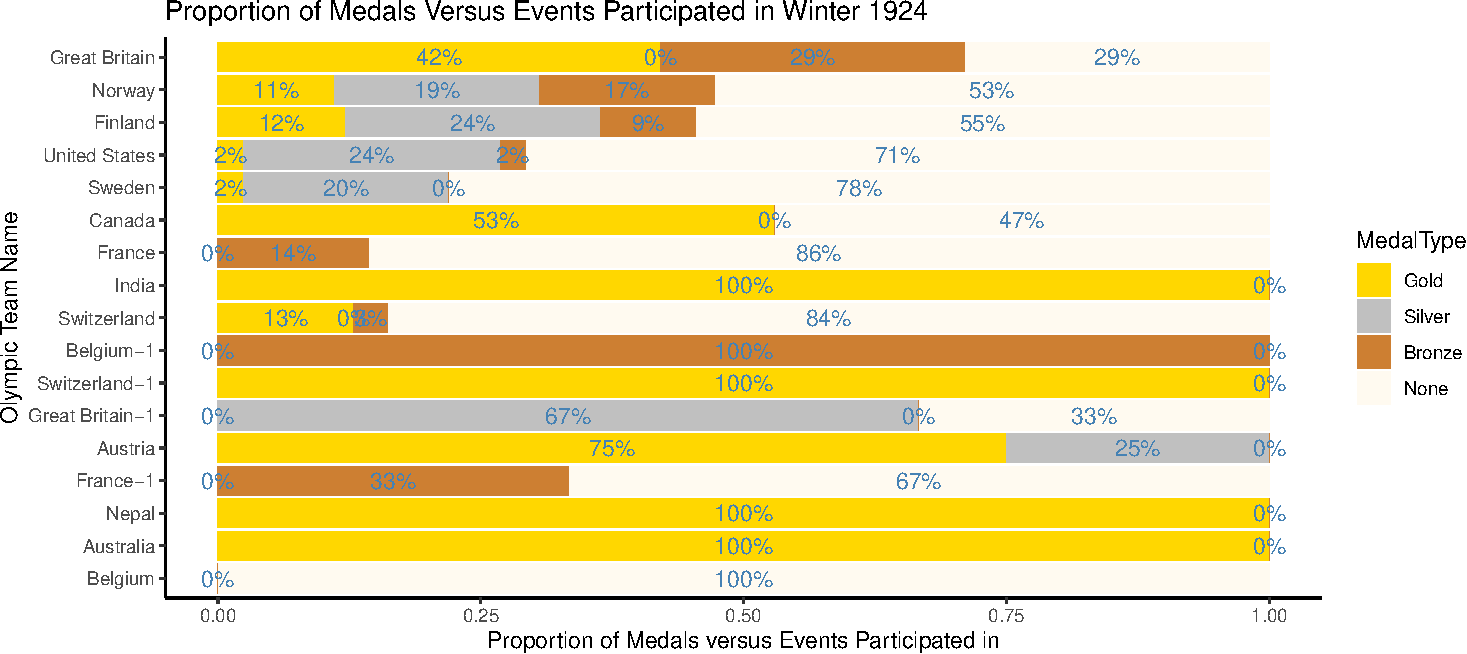
\includegraphics[keepaspectratio]{C:/Final/report/DSAA811_Final_files/figure-latex/medalProp3-1.pdf}}
\caption{\label{fig:medalProp3}Proportion of medals in relation to the events entered by teams in the Winter 1924 Olympics for the top 17 teams}
\end{figure}

\begin{figure}
\centering
\pandocbounded{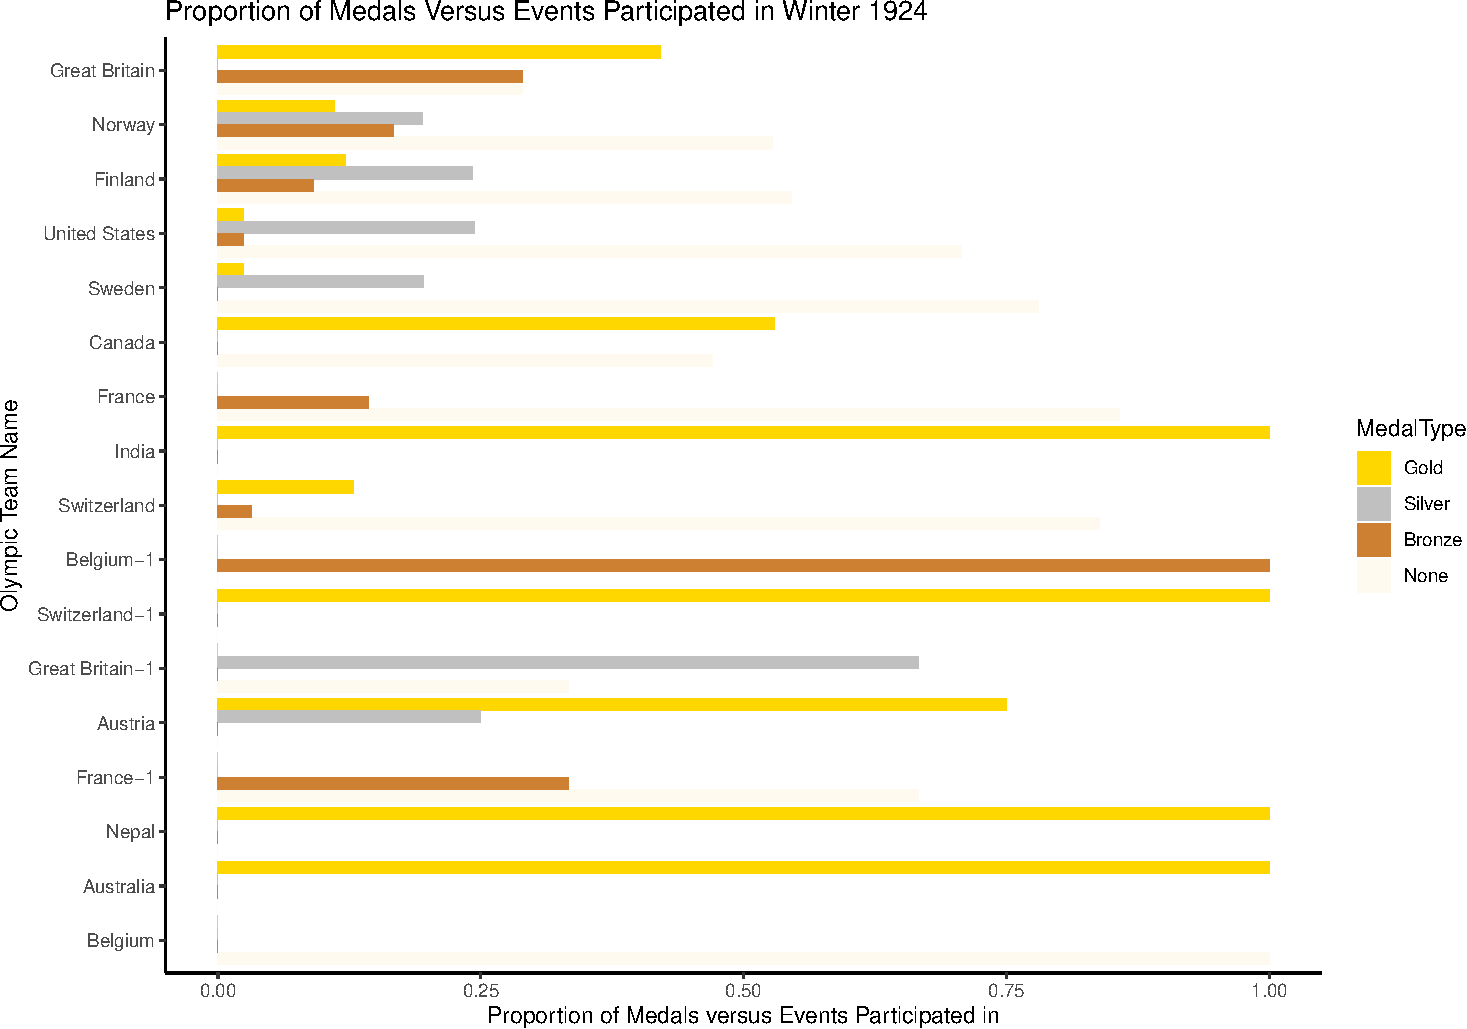
\includegraphics[keepaspectratio]{C:/Final/report/DSAA811_Final_files/figure-latex/medalProp4-1.pdf}}
\caption{\label{fig:medalProp4}Proportion of medals in relation to the events entered by teams in the Winter 1924 Olympics for the top 17 teams}
\end{figure}

Sticking to the the Summer Olympics in 1896. Table \ref{tab:SummerBreakDownWinners3} tells us the number of athletes that were sent by each team. Greecce sent 101 athletes, whereas Sweeden, Australia, and Italy sent only 1 person. Germany sent 19 athletes, however they recieved 24 gold medals, more than those members on the team. Visually using Figure \ref{fig:medalPropAth}, it is easy to see that Sweeden had a 500\% sucess rate of winning no medals. In other terms, there were 5 events that were entered where no-one on the team won. Australia had a 200\% success rate meaning that every athlete on the team brought home 2 gold medals. Removing the numbers from the bars and comparing these figures with that of \ref{tab:SummerBreakDownWinners3} we can see very similar trends. There is no evidence to suggest sending less athletes brings home any more or any less medals.

\begin{table}[H]
\centering
\caption{\label{tab:SummerBreakDownWinners3}Medal allocation for 1896 Summer Olympic Games}
\centering
\fontsize{7}{9}\selectfont
\begin{tabular}[t]{lrrrrr}
\toprule
Team & Gold & Silver & Bronze & Events & AthletesSent\\
\midrule
\cellcolor{gray!10}{Greece} & \cellcolor{gray!10}{10} & \cellcolor{gray!10}{16} & \cellcolor{gray!10}{18} & \cellcolor{gray!10}{140} & \cellcolor{gray!10}{101}\\
Germany & 24 & 5 & 2 & 93 & 19\\
\cellcolor{gray!10}{United States} & \cellcolor{gray!10}{11} & \cellcolor{gray!10}{7} & \cellcolor{gray!10}{2} & \cellcolor{gray!10}{27} & \cellcolor{gray!10}{14}\\
France & 5 & 4 & 2 & 26 & 12\\
\cellcolor{gray!10}{Great Britain} & \cellcolor{gray!10}{2} & \cellcolor{gray!10}{3} & \cellcolor{gray!10}{2} & \cellcolor{gray!10}{23} & \cellcolor{gray!10}{10}\\
\addlinespace
Denmark & 1 & 2 & 3 & 15 & 3\\
\cellcolor{gray!10}{Hungary} & \cellcolor{gray!10}{2} & \cellcolor{gray!10}{1} & \cellcolor{gray!10}{3} & \cellcolor{gray!10}{18} & \cellcolor{gray!10}{7}\\
Austria & 2 & 1 & 2 & 8 & 3\\
\cellcolor{gray!10}{Switzerland} & \cellcolor{gray!10}{1} & \cellcolor{gray!10}{2} & \cellcolor{gray!10}{0} & \cellcolor{gray!10}{8} & \cellcolor{gray!10}{3}\\
Australia & 2 & 0 & 0 & 4 & 1\\
\addlinespace
\cellcolor{gray!10}{Australia/Great Britain} & \cellcolor{gray!10}{0} & \cellcolor{gray!10}{0} & \cellcolor{gray!10}{2} & \cellcolor{gray!10}{2} & \cellcolor{gray!10}{2}\\
Ethnikos Gymnastikos Syllogos & 0 & 0 & 2 & 2 & 2\\
\cellcolor{gray!10}{Great Britain/Germany} & \cellcolor{gray!10}{2} & \cellcolor{gray!10}{0} & \cellcolor{gray!10}{0} & \cellcolor{gray!10}{2} & \cellcolor{gray!10}{2}\\
Greece-1 & 0 & 2 & 0 & 2 & 2\\
\cellcolor{gray!10}{Greece-2} & \cellcolor{gray!10}{0} & \cellcolor{gray!10}{0} & \cellcolor{gray!10}{0} & \cellcolor{gray!10}{2} & \cellcolor{gray!10}{2}\\
\addlinespace
Greece-3 & 0 & 0 & 0 & 2 & 2\\
\cellcolor{gray!10}{Italy} & \cellcolor{gray!10}{0} & \cellcolor{gray!10}{0} & \cellcolor{gray!10}{0} & \cellcolor{gray!10}{1} & \cellcolor{gray!10}{1}\\
Sweden & 0 & 0 & 0 & 5 & 1\\
\bottomrule
\end{tabular}
\end{table}

\begin{figure}
\centering
\pandocbounded{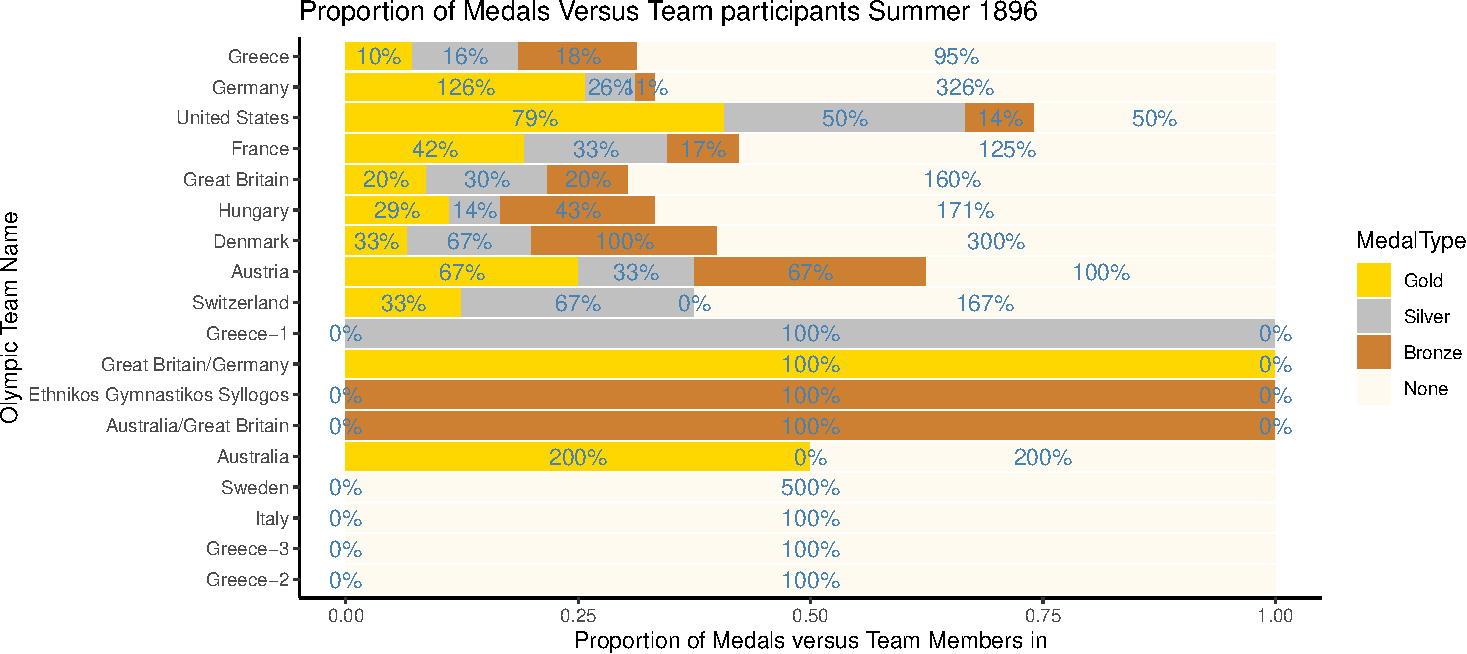
\includegraphics[keepaspectratio]{C:/Final/report/DSAA811_Final_files/figure-latex/medalPropAth-1.pdf}}
\caption{\label{fig:medalPropAth}Proportion of medals in relation to the number of athletes entered by teams in the Summer 1896 Olympics}
\end{figure}

Finally, I explore the last question of the research \emph{3) What are the sports that have the most events and as such the highest potential to win a medal? Has this always been the case? What are the future predictions for medal obtainment moving into the next Olympic games in both Summer and Winter Olympics?}

Figure \ref{fig:SportTrends} takes a sample of 16 Olympic events from the summer games. This plot shows the trend lines for the number of competitors that competed in each year of the olympics in those selected sports. Ruling and governing bodies such as the NOC are in charge of keeping the competition fair, and as such govern the numbers of athletes competing. We can tell from this plot that there is an increasing number of athletes that are participating in Athletics. Gymnastics showed a major increase but has taken a downward turn in athletes to now having steady numbers. There is no evidence to suggest specialising in one type of sport over another increases you chance to be selected to participate or even bring home the covenant medals.

\begin{figure}
\centering
\pandocbounded{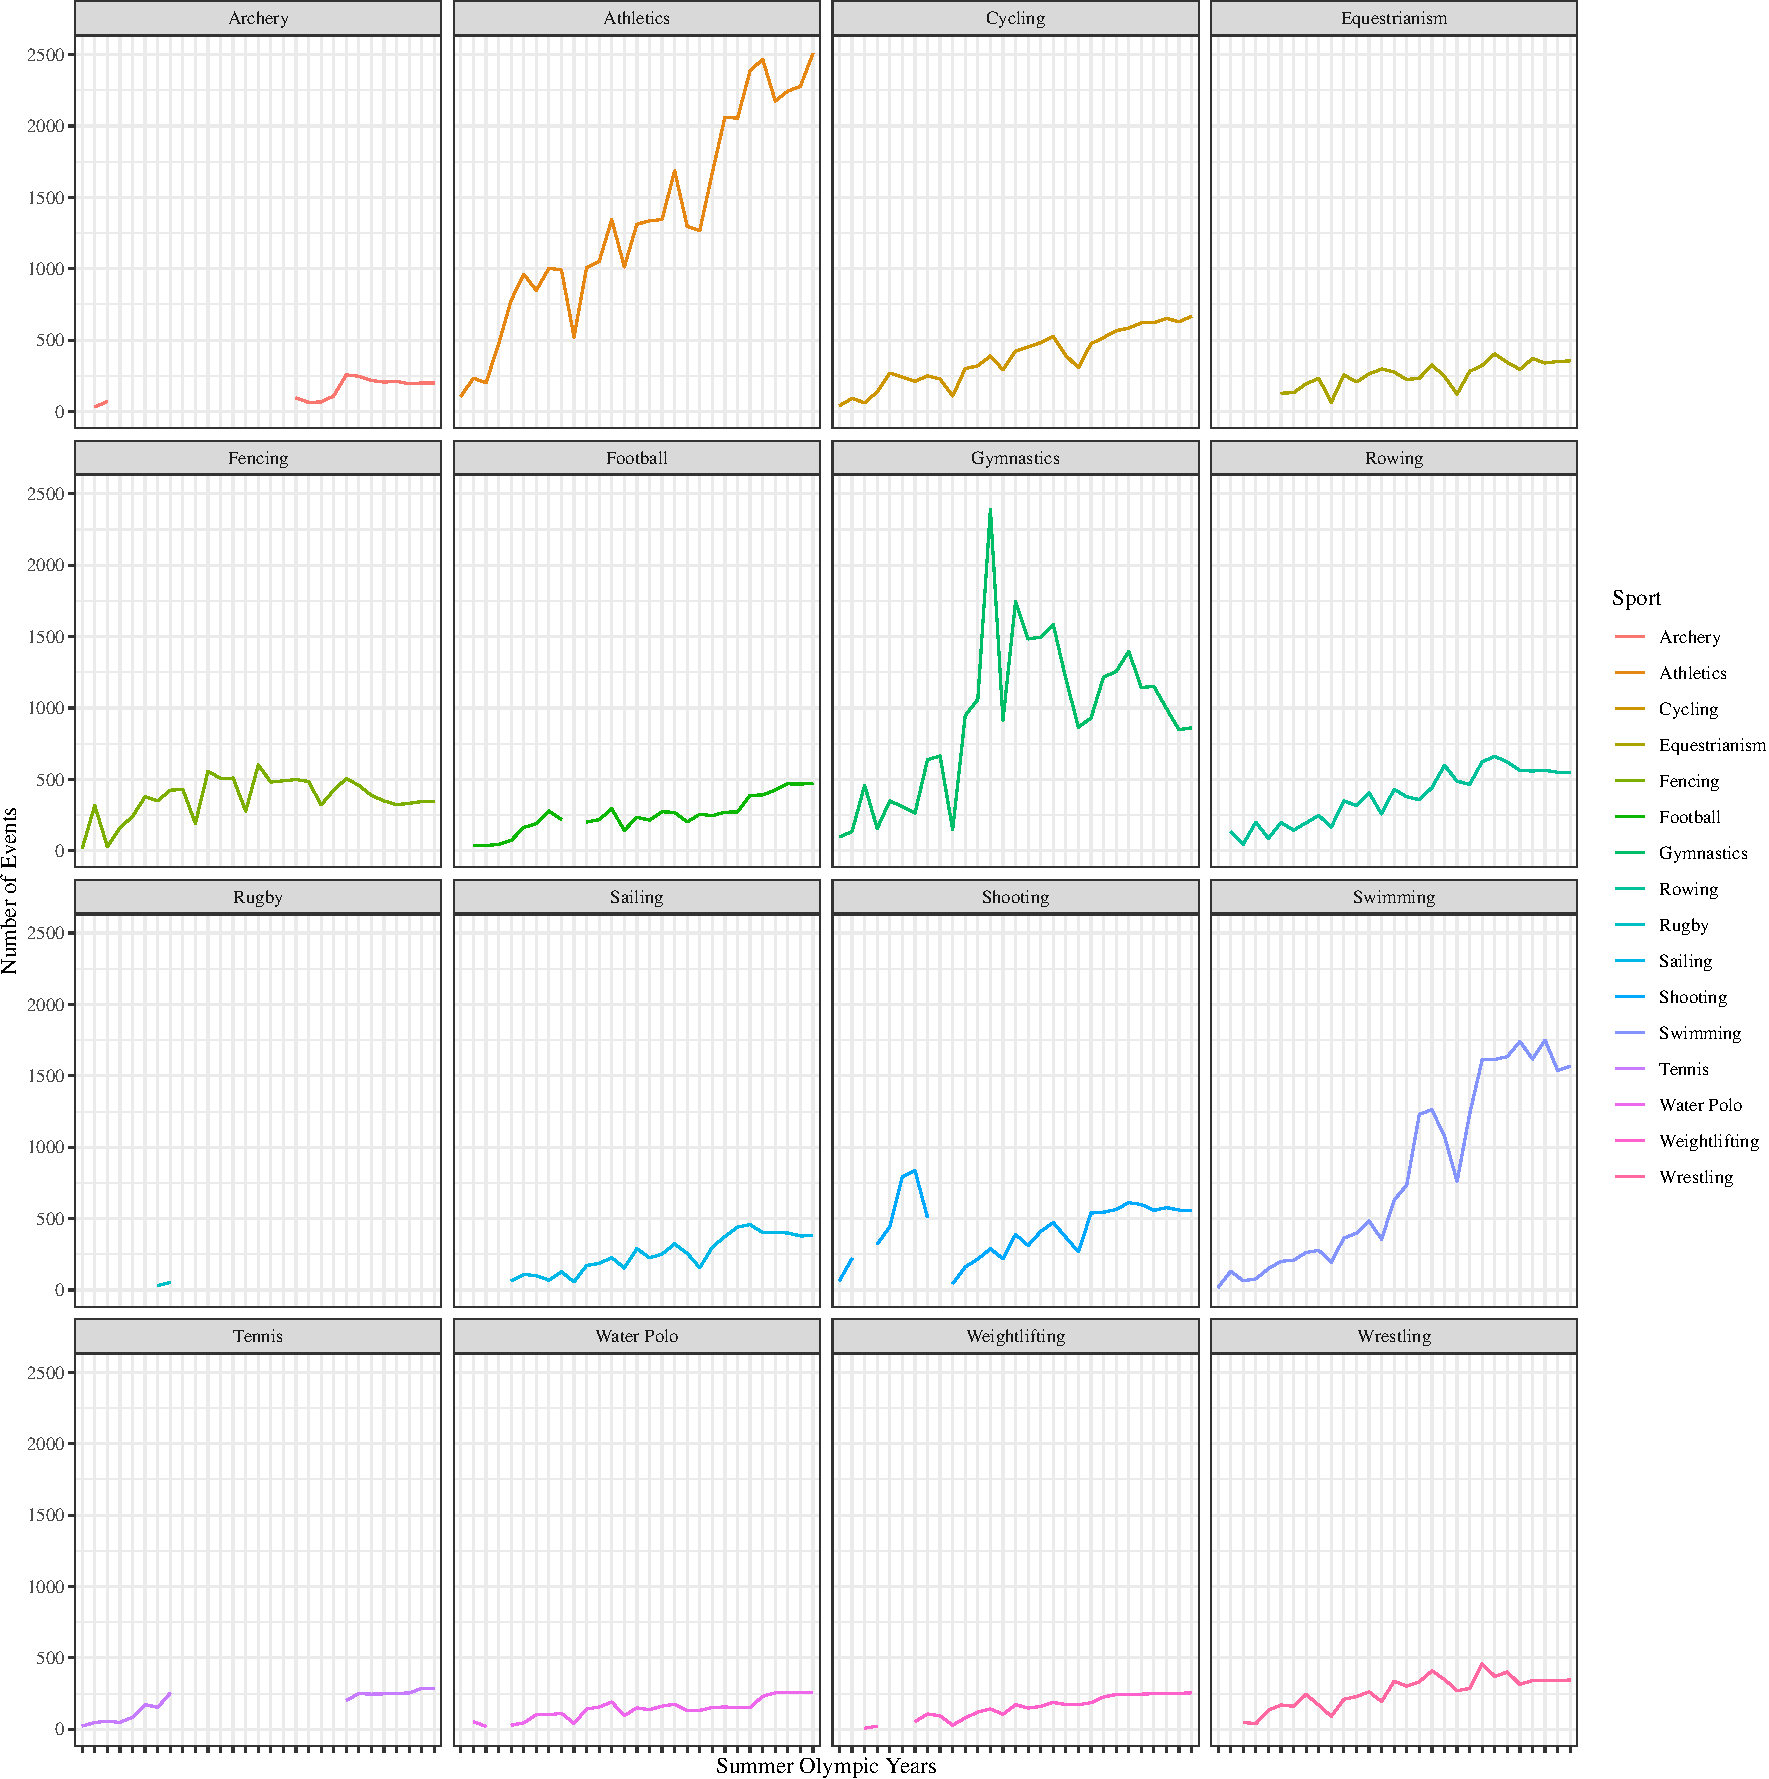
\includegraphics[keepaspectratio]{C:/Final/report/DSAA811_Final_files/figure-latex/SportTrends-1.pdf}}
\caption{\label{fig:SportTrends}Trend lines of Summer Olympic sport event numbers since 1896}
\end{figure}

\newpage

\section*{Conclusion / Discussion}\label{conclusion-discussion}
\addcontentsline{toc}{section}{Conclusion / Discussion}

In conclusion, I looked into the changes in the Olympic games from their inception in 1896 for the Summer Olympic games and in 1924 Winter Olympics. I found that there are an increasing number of sports being introduced into both types of games. There was some sports that are no longer participated in such as Military Ski Patrol. I discovered that the number of medals awarded is not proportionate to the number of athletes that you send. Sending less athletes and having them compete in multiple events did not equate to less medals if those athletes are up to the job. There is a trend towards increasing participation in Athletic events, whilst larger sporting events such as swimming, and gymnastics have quite a large participation and have stabalised in participation numbers.

\newpage

\#Session Information \{-\}

\begin{Shaded}
\begin{Highlighting}[]
\FunctionTok{sessionInfo}\NormalTok{()}
\end{Highlighting}
\end{Shaded}

\begin{verbatim}
## R version 4.5.0 (2025-04-11 ucrt)
## Platform: x86_64-w64-mingw32/x64
## Running under: Windows 11 x64 (build 26100)
## 
## Matrix products: default
##   LAPACK version 3.12.1
## 
## locale:
## [1] LC_COLLATE=English_United States.utf8 
## [2] LC_CTYPE=English_United States.utf8   
## [3] LC_MONETARY=English_United States.utf8
## [4] LC_NUMERIC=C                          
## [5] LC_TIME=English_United States.utf8    
## 
## time zone: Australia/Sydney
## tzcode source: internal
## 
## attached base packages:
## [1] stats     graphics  grDevices utils     datasets  methods   base     
## 
## other attached packages:
##  [1] magrittr_2.0.3   maps_3.4.2.1     sjmisc_2.8.10    kableExtra_1.4.0
##  [5] sf_1.0-21        lmerTest_3.1-3   lme4_1.1-37      Matrix_1.7-3    
##  [9] lubridate_1.9.4  forcats_1.0.0    stringr_1.5.1    purrr_1.0.4     
## [13] readr_2.1.5      tibble_3.2.1     tidyverse_2.0.0  ggplot2_3.5.2   
## [17] dplyr_1.1.4      tidyr_1.3.1      tinytex_0.57     knitr_1.50      
## 
## loaded via a namespace (and not attached):
##  [1] gtable_0.3.6        xfun_0.52           insight_1.3.0      
##  [4] lattice_0.22-6      tzdb_0.5.0          numDeriv_2016.8-1.1
##  [7] vctrs_0.6.5         tools_4.5.0         Rdpack_2.6.4       
## [10] generics_0.1.4      proxy_0.4-27        pkgconfig_2.0.3    
## [13] KernSmooth_2.23-26  RColorBrewer_1.1-3  lifecycle_1.0.4    
## [16] compiler_4.5.0      farver_2.1.2        textshaping_1.0.1  
## [19] htmltools_0.5.8.1   class_7.3-23        yaml_2.3.10        
## [22] pillar_1.10.2       nloptr_2.2.1        MASS_7.3-65        
## [25] classInt_0.4-11     reformulas_0.4.1    boot_1.3-31        
## [28] nlme_3.1-168        sjlabelled_1.2.0    tidyselect_1.2.1   
## [31] digest_0.6.37       stringi_1.8.7       bookdown_0.43      
## [34] labeling_0.4.3      splines_4.5.0       rprojroot_2.0.4    
## [37] fastmap_1.2.0       grid_4.5.0          cli_3.6.5          
## [40] e1071_1.7-16        withr_3.0.2         scales_1.4.0       
## [43] timechange_0.3.0    rmarkdown_2.29      hms_1.1.3          
## [46] evaluate_1.0.3      rbibutils_2.3       viridisLite_0.4.2  
## [49] rlang_1.1.6         Rcpp_1.0.14         glue_1.8.0         
## [52] DBI_1.2.3           xml2_1.3.8          svglite_2.2.1      
## [55] rstudioapi_0.17.1   minqa_1.2.8         R6_2.6.1           
## [58] systemfonts_1.2.3   units_0.8-7
\end{verbatim}

\newpage

\section*{Bibliography}\label{bibliography}
\addcontentsline{toc}{section}{Bibliography}

\phantomsection\label{refs}
\begin{CSLReferences}{1}{0}
\bibitem[\citeproctext]{ref-bansal_2021_olympics_}
Bansal, Harsh. 2021. {``Olympics\_.''} Kaggle.com. \url{https://www.kaggle.com/datasets/harshbansal27/olympics}.

\bibitem[\citeproctext]{ref-a262588213843476_2021_countries}
Ferlet, Patrice. 2021. {``Countries Coordinates with Longitude and Latitude.''} Gist. \url{https://gist.github.com/metal3d/5b925077e66194551df949de64e910f6}.

\bibitem[\citeproctext]{ref-OxfordStudy}
Flyvbjerg, Bent, Allison Stewart, and Alexander Budzier. 2016. {``The Oxford Olympics Study 2016: Cost and Cost Overrun at the Games.''} \emph{Saïd Business School Working Papers}, July. \url{https://doi.org/10.2139/ssrn.2804554}.

\bibitem[\citeproctext]{ref-heazlewood_2006_prediction}
Heazlewood, Timothy. 2006. {``Prediction Versus Reality: The Use of Mathematical Models to Predict Elite Performance in Swimming and Athletics at the Olympic Games.''} \emph{Journal of Sports Science \& Medicine} 5 (December): 480. \url{https://pmc.ncbi.nlm.nih.gov/articles/PMC3861753/}.

\bibitem[\citeproctext]{ref-a2020_olympic}
History, Parramatta, and Heritage. 2020. {``Olympic Games - a Brief History \textbar{} Parramatta History and Heritage.''} Nsw.gov.au. \url{https://historyandheritage.cityofparramatta.nsw.gov.au/research-topics/events/olympic-games-brief-history}.

\bibitem[\citeproctext]{ref-keating_2025_kaggle}
Keating, Nate, Jeff Moser, William Cukierski, Jerad Rose, Myles O'Neill, Risdal Meg, Meghan O'Connell, et al. 2025. {``Kaggle: Your Home for Data Science.''} Kaggle.com. \url{https://www.kaggle.com/}.

\end{CSLReferences}

\end{document}
